\item
\mbox{}
\begin{center}
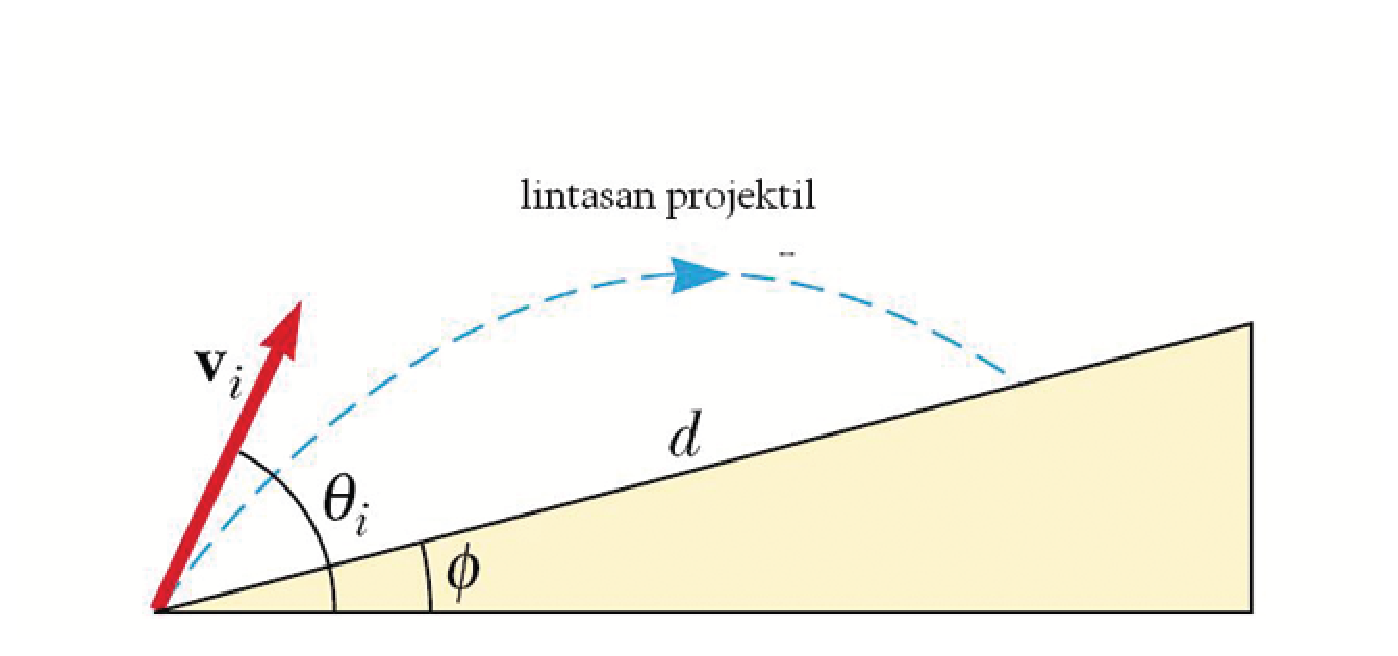
\includegraphics [scale=0.3]{./latex/eps/1_4_1_image_1.eps}
\end{center}a. Projektil dilontarkan pada bidang miring dengan sudut $\phi$ dengan kecepatan awal $v$ dan sudut $\theta$ terhadap horizontal seperti pada gambar. Tunjukan bahwa projektil akan menempuh jarak $d$, dimana $d$ =
\begin{equation*}
        d= \frac{2 v \cos \left(\theta\right) \sin\left(\theta-\phi\right)}{g \cos^2\left(\theta\right)}
\end{equation*}

b. Berapa nilai $\theta$ supaya $d$ maksimum dan berapa nilai maksimum tersebut ?

